%種々宣言
\documentclass[12pt, oneside]{jreport}   	
\usepackage{geometry}                		
\geometry{letterpaper}                   		
\usepackage[dvipdfmx]{graphicx}				
\usepackage{listings,jlisting}										
\usepackage{amssymb}
\usepackage{ascmac}
\usepackage{here}

%文書開始
\begin{document}


%タイトルページ
\begin{center}

{\Huge ソフトウェア要求仕様書}

\vspace{15mm}

{\huge 「DiscussionVisualizerの改良」}

\vspace{30mm}

{\Large 東京工業大学工学部情報工学科 佐伯研究室}

\vspace{10mm}

{\large 高橋 碧 (Takahashi Aoi)}

\vspace{1mm}

{\large 梅田 侑 (Umeda Yuu)}

\vspace{10mm}

{\large 2017年 5月22日}

\end{center}

\newpage 


%目次ページ
\tableofcontents
\clearpage


%本文開始

\chapter{仕様書の概要}

	\section{目的}
	本要求仕様書は、Issue Tracking System (ITS) 上のissueの議論の流れを構造化して視覚的に表示するツールである「DiscussionVisualizer」を改良することによって、ITS利用者が議論の流れをより把握しやすくするために、「DiscussionVisualizer」が満たすべき要求やその理由、制約などを明らかにすることを目的とする。本ツールの開発者及びステークホルダ、特に本ツールの使用者を対象読者とする。
	
	\section{範囲}
	本ツールはITS利用者のissueの内容把握を支援する。また、本ツールでのITSはJIRAを対象とし、JIRAにあるissueに関しての議論構造の生成や、編集を行う。本ツールを利用することで、issue上の議論の流れを視覚的に捉えることができるという利点がある。本ツールに対して、ユーザビリティを向上させることでその利点を最大限生かせるようにする。さらに、協調作業支援機能 (CSCW) を付与することで、個人でのissueの理解だけでなく、複数人でのissueの理解を共有できるようにする。
	
	これらの内容を満たすことで、「DiscussionVisualizer」の実用性の向上を図ることが目的である。

	\newpage
	
	\section{用語定義}
	%未実装
	\begin{table}[htb]
		\begin{center}
		\caption{用語定義}
		\small
  		\begin{tabular}{|c|c|} \hline
    		用語 & 定義 \\ \hline \hline
    		DiscussionVisualizer & \shortstack{昨年度、佐伯研究室に所属していた大内さんが作成した\\issue上の議論構造可視化と理解支援をするツールのこと}  \\ \hline
		Issue Tracking System (ITS) & 課題管理システムのこと \\ \hline
		JIRA & ITSのツールの一つ \\ \hline
		Ruby on Rails & Webアプリケーションフレームワークの一つ \\ \hline
		\shortstack{Model View Controller \\(MVC)} & \shortstack{アプリケーションソフトウェアを実装するためのデザインパターンの一つ\\ Ruby on Railsではこのデザインパターンが採用されている} \\ \hline
		Graphviz & グラフを描画するツール \\ \hline
		プロジェクト & JIRA上に設けられているプロジェクトのこと  \\ \hline
		issue & JIRA上に設けられているissueのこと。プロジェクトごとに存在する  \\ \hline
    		議論構造 & issue上の議論をGraphvizを用いて木構造として可視化したグラフのこと  \\ \hline
    		\shortstack{Computer Supported \\ Cooperative Work (CSCW)} & 協調作業支援機能。複数人でツールを利用し、作業を進めるための機能  \\ \hline
    		コメント & \shortstack{JIRAのissue上のコメントを抽出し、議論構造と同時に\\「DiscussionVisualizer」に表示されているもの}  \\ \hline
		タグ付け & コメントに対して、特定のタグを付けること  \\ \hline
		フィルタリング & コメントに付いているタグに従って、コメントの一部を表示する機能  \\ \hline
    		議論参加者名 & JIRAの表示名  \\ \hline
  		\end{tabular}
		\normalsize
  		\end{center}
	\end{table}	
	
	\newpage
	
	\section{概要}
	本要求仕様書では、第2章の全容で、要求分析の結果考えられる現状の問題点に関して、具体的に確認する。また本ツールの機能の概要を記述する。第3章の要求仕様では、本ツールの詳細な機能の仕様について記述する。
	

\chapter{全容}

	\section{製品の背景}
	現状のツールでは、個人でのissue上の議論構造の可視化を目的としている。また、元の「DiscussionVisualizer」の実装期間の関係で、機能はきちんと実装されているが、実際にツールとして使いやすいものとは言えない。そのため以下の問題点が存在する。
	
	現状のツールに関する問題点は、大きくCSCWとユーザビリティである。
	
	CSCWについて、現状では個人でのissue管理を目的としてツールが作られているため、共同でissue管理をすることができない。このことは、複数人でissue管理をしたい場合には致命的な問題点である。
	
	ユーザビリティについて、現状では議論構造を編集しづらく、タグ付けをしたコメントに対するフィルタリングの種類が少ないことによる、コメントの整理のしづらさがある。他には、issueが全て同じ階層で一覧になっているため、多くのissueを管理する際にとても見づらい。また、JIRAではissueごとにissue間の関係が定義されているが、その関係を「DiscussionVisualizer」では抽出できていないため、管理したいissueがどのissueと関係があるのか分からない。このような問題点がある。
	
	これらの問題点を解決するために、いくつかの機能を実装する。
	
	\section{製品機能}
	ユーザビリティに関して、本ツール改良案では以下の4つの機能により、上記の問題点を解決する。
	\begin{itemize}
		\item 議論構造の編集・整理のユーザビリティ向上
		\\
		 議論構造の編集のしやすさを向上させ、編集のコストを軽減させる。
		\item タグに対するフィルタリングの種類の追加
		\\
		 フィルタリングの種類を増やすことで、タグ付けを最大限生かし、コメントを整理しやすくする。
		\item プロジェクトごとのグループ化
		\\
		 issueを同じ階層で一覧にするのではなく、プロジェクトごとにissueを一覧にすることで、issueが多くなった場合にも見やすさを維持する。
		\item 複数issue間の関係の可視化
		\\
		 JIRAに元々存在する関係を抽出し、表示することで、issue間の関係を分かりやすくする。
	\end{itemize}
	
	また、自動でタグ付けをする機能を拡張し、ユーザが任意の議論参加者に対してタグ名を登録し、その議論参加者に自動でタグ付けをする機能も実装する。
	\\
	
	CSCWに関して、本ツール改良案では以下の4つの機能により、上記の問題点を解決する。
	\begin{itemize}
		\item ユーザ名の追加
		\\
		 アカウントに対して、ユーザ名を追加し共同作業の際に自身を特定する名前を設ける。
		\item プロジェクト/issue一覧の共有
		\\
		 プロジェクト/issue一覧を共有することで、複数人で共有しながら、プロジェクト/issueを追加したり閲覧できたりする。
		\item 議論構造の共有
		\\
		 議論構造を共有することで、複数人で共有しながら、議論構造を編集したり、整理できたりする。
		\item issueごとに担当者・状態の管理
		\\
		 issueごとに担当者や状態を管理することで、複数人で共有しながら、issueを管理できる。
	\end{itemize}

	\section{仮定および依存性}
	本ツールでは、ITSとしてJIRAを利用していること、また元の「DiscussionVisualizer」を利用することが可能である環境を仮定している。具体的には、Ruby on Rails 5.0.0、ruby 2.3.1、graphvizがインストールされている必要がある。

\chapter{要求仕様}

	\section{外部インターフェイス要求}
		
		\subsection{ユーザインターフェイス要求}

		初回利用時には、新規アカウントを作成する。そうでない場合にはログインをして本ツールを利用する。新規アカウント作成の場合には、ユーザ名、メールアドレス、パスワードを入力する必要がある。ログインの場合には、メールアドレスとパスワードを入力する必要がある。ログイン後、新規プロジェクト追加のページから新規プロジェクトを追加し、JiraのissueのURLを新規issue作成のページから入力することで議論構造を自動生成し、その議論構造に対してユーザは閲覧・編集を行うことができる。また、issue一覧ページからissueを閲覧できる。ログイン時にはどのページからもログアウトをすることができ、ログアウトをした場合には、新規アカウント作成もしくはログインをするページに戻ることができる。

	
	\section{機能要求}
	ここでは、具体的な機能について記述する。また、機能は実装の優先順位順に記述していく。1ヶ月の間で実装をするというスケジュールを考慮し、[最低限機能]と[発展機能]に機能を分類する。
	
		\subsection{[最低限機能] CSCWの向上}
		\begin{itemize}
			\item ユーザ名を追加
			\\ \\
			新規アカウント登録をする際に、ユーザ名を追加する欄を作り、アカウント情報にユーザ名を追加する。これにより、issueごとに担当者を追加する際にも、現在アカウント登録されているユーザ名の中から担当者を選択することが可能になる。他にも、issue一覧ページにユーザ名を表示することで、自分のログインしたアカウントが本当に自分のアカウントであるのかというのも明確にわかるようになり、共同作業をする際には便利である。以下に、この機能を実装した場合の画面例を示す。
			
			\begin{figure}[H]
			\centering
			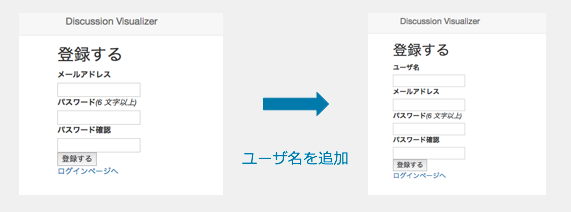
\includegraphics[width=17cm,bb=520 300 -200 27]{UserName1.png}
			\caption{新規アカウント登録ページ}
			\end{figure}
			
			\begin{figure}[H]
			\centering
			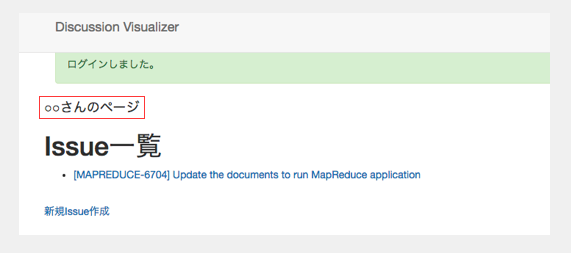
\includegraphics[width=17cm,bb=470 300 -200 27]{UserName2.png}
			\caption{issue一覧ページにユーザ名を表示}
			\end{figure}
		
			\item プロジェクト/issue一覧の共有
			\\ \\
			複数人がissueを管理していても、そのissue一覧が共有されなければ共同で作業を進めることはできない。そのために、他の誰かがissueを追加した場合に、自分のissue一覧にそのissueが追加されていなければいけない。そのための機能である。すべてのissueはプロジェクトごとに分類され、自分のissue一覧のページに表示される。担当者機能を実装する場合、自分が担当しているissueに絞って表示できる機能を実装する。以下に修正前と修正後の画面例を示す。
			\begin{figure}[H]
			\centering
			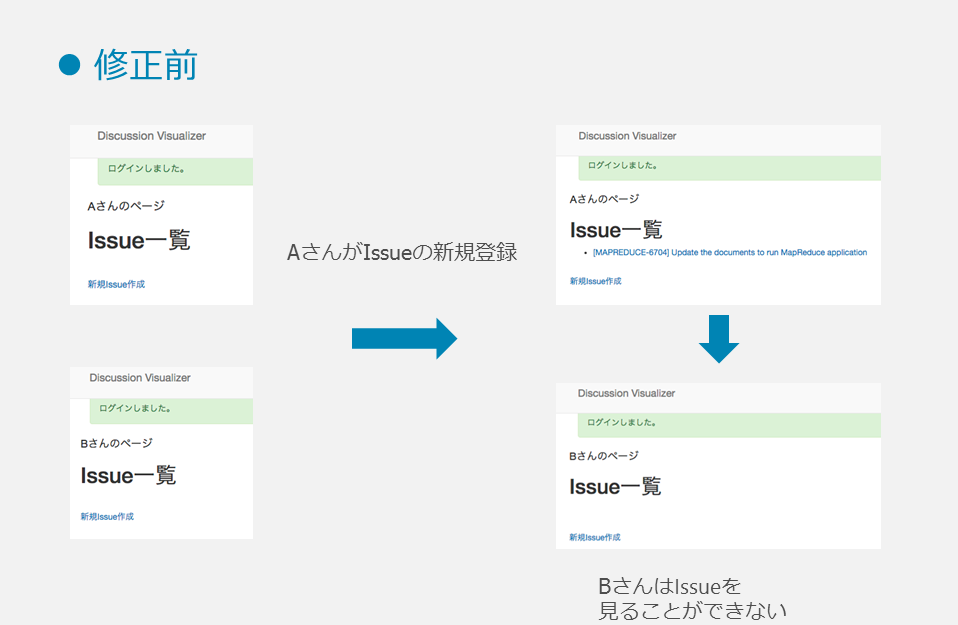
\includegraphics[width=17cm,bb=200 300 -200 27]{IssShare_before.PNG}
			\caption{プロジェクト/issue一覧の共有(修正前)}
			\end{figure}
			\begin{figure}[H]
			\centering
			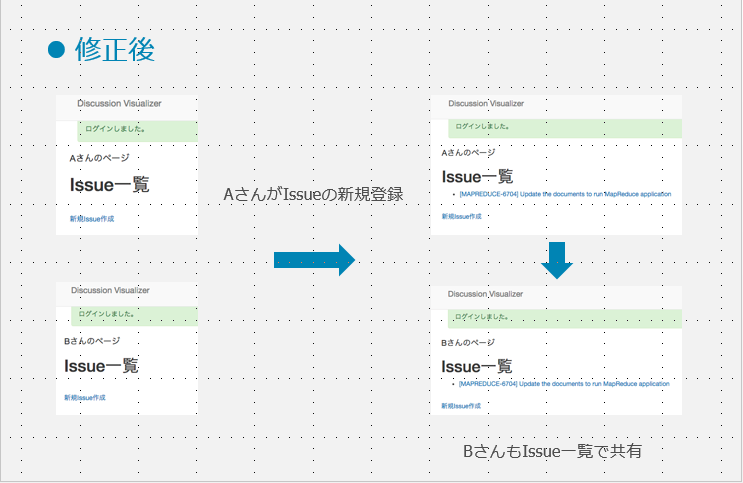
\includegraphics[width=17cm,bb=200 300 -200 27]{IssShare_after.PNG}
			\caption{プロジェクト/issue一覧の共有(修正後)}
			\end{figure}

		
			\item 議論構造の共有
			\\ \\
			プロジェクト/issue一覧の共有と同様に、議論構造に関しても、議論構造の変更が共有されていなければ、共同で作業を進めることはできない。そのための機能である。以下に、修正前と修正後の画面例を示す。
			
			\begin{figure}[H]
			\centering
			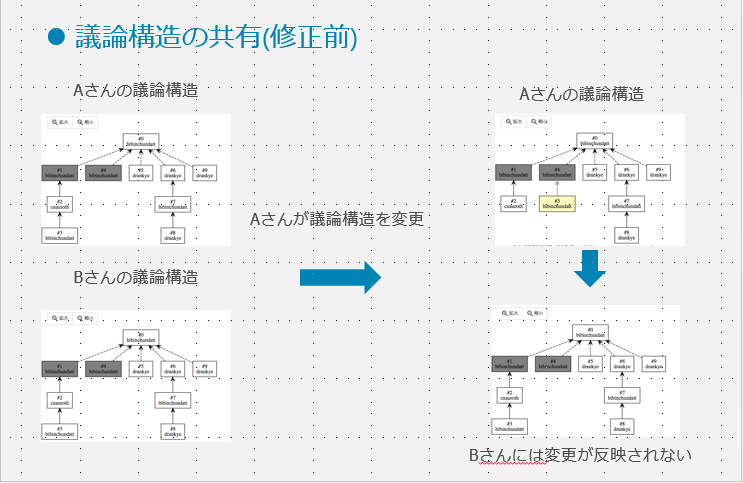
\includegraphics[width=17cm,bb=200 300 -200 27]{graphedit_before.PNG}
			\caption{議論構造の共有(修正前)}
			\end{figure}
						\begin{figure}[H]
			\centering
			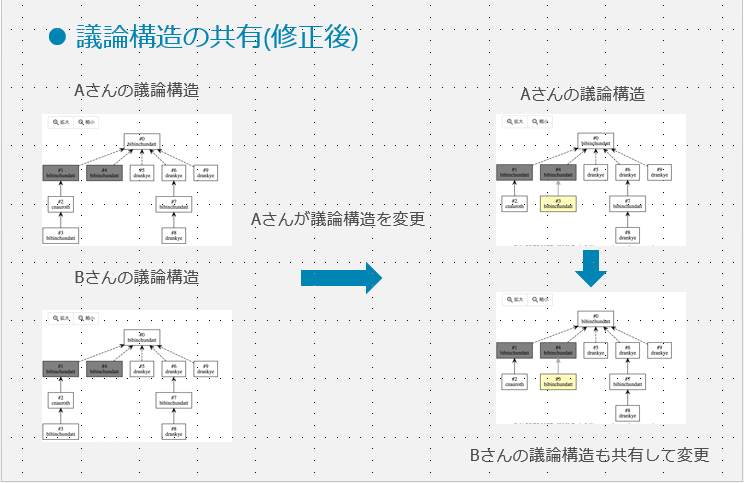
\includegraphics[width=17cm,bb=200 300 -200 27]{graphedit_after.PNG}
			\caption{議論構造の共有(修正後)}
			\end{figure}
			
		\end{itemize}
		
		共有に関して、現在の実装の説明では、ほぼ同時に複数ユーザが編集をした際に編集のコンフリクトが起こる可能性があるが特に対策は行わないため、注意して運用する。もし同時に二人のユーザーが議論構造を編集した場合、後の編集が反映される。
		
		\subsection{[最低限機能] プロジェクトごとのグループ化}
		多くのissueが追加された場合の見づらさを防止するために、issueをプロジェクトごとに管理する。具体的には、プロジェクトを手動で追加し、プロジェクトごとにissueを追加できるようにする。そうすることで、プロジェクトごとにissueをグループ化でき、見やすさが向上する。以下に、画面例を示す。
		
		\begin{figure}[H]
		\centering
		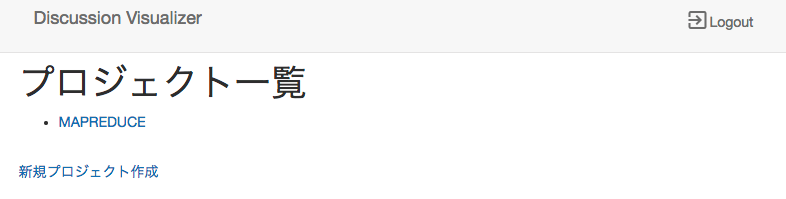
\includegraphics[width=17cm,bb=700 300 -200 27]{ProjectList.png}
		\caption{プロジェクト一覧ページ}
		\end{figure}
		
		まず、今まではissue一覧であったページをプロジェクト一覧ページに変える。こうすることで、まず閲覧したいプロジェクトを選択することになる。
			
		\begin{figure}[H]
		\centering
		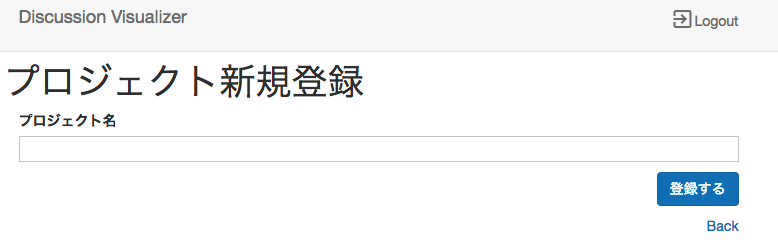
\includegraphics[width=17cm,bb=500 300 -200 27]{ProjectAdd.png}
		\caption{プロジェクト新規登録ページ}
		\end{figure}
		
		また、プロジェクト一覧ページでは新規にプロジェクトを追加することもできる。
		
		\begin{figure}[H]
		\centering
		\includegraphics[width=17cm,bb=500 300 -200 27]{ProjectissueList.png}
		\caption{プロジェクトごとのissue一覧}
		\end{figure}
		
		プロジェクト一覧ページのプロジェクトを選択すると、そのプロジェクト内のissue一覧を閲覧することができる。また、issueを追加したい場合には、プロジェクト内の新規issue作成ボタンから、プロジェクトごとにissueを追加することができる。さらに、プロジェクト一覧ページにも新規issue作成ページを用意し、プロジェクト一覧ページの新規issue作成ページから新規issueを作成した場合、issue名などからプロジェクト名を自動で判定して適切なプロジェクトに割り当てる。
		
		\subsection{[最低限機能] プロジェクトごとに自動タグ付けを登録}
		現在では、issueを登録した際に、コメントに自動でタグ付けがされるようになっている。しかし、そのタグ付けはあらかじめ用意されているタグ付けのみである。そのため、上に述べたプロジェクトごとに、自動で、タグ付けをするものを登録できるようにする。登録ページでは、自動でタグ付けをしたい議論参加者名と、その議論参加者名(JIRAの表示名)にどのようなタグ付けをしたいかを入力して登録する。登録すると、過去に登録したすべてのissueについて新しい自動タグ付け規則によってタグをつける。また、タグを削除した場合、過去に付けたタグも削除されるものとする。以下に、画面例を示す。
		\begin{figure}[H]
		\centering
		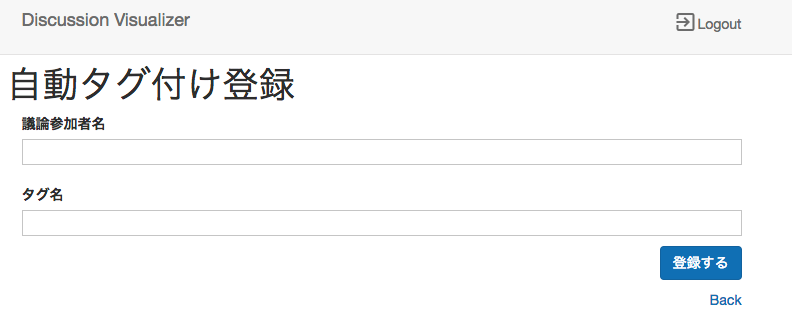
\includegraphics[width=17cm,bb=500 300 -200 27]{TagAdd.png}
		\caption{自動タグ付け登録ページ}
		\end{figure}
		
		画面例として示しているが、実際にはもう少しユーザビリティを向上したいと考えている。この画面では一度に登録できるのが1組だけだが、そうではなく複数の登録をまとめてできるような入力フォームにすべきである。具体的には、カンマ区切りの入力、ボタンによる入力フォームの追加等が挙げられる。

		\subsection{[発展機能] タグに対するフィルタリングの種類の追加}
		現状では、フィルタリング機能はタグを一つ選択するとそのタグが付いているコメントがフィルタリングされる。しかし、そのようなフィルタリングだけでなく、選択したタグを持っているコメントだけを非表示にするフィルタリングや、複数タグを選択してフィルタリングをすることもできるようにする。

		\subsection{[発展機能] 複数issue間の関係の可視化}
		概要でも記述した通り、JIRAではissue間に関係が存在する。その関係を現状では取り込むことができておらず、どのissueとどのissueが関係し合っているのかを確認できない。このことを改善するために、issueごとにJIRAでのissue間の関係を表示するような機能をつける。以下に、画面例を示す。
		
		\begin{figure}[H]
		\centering
		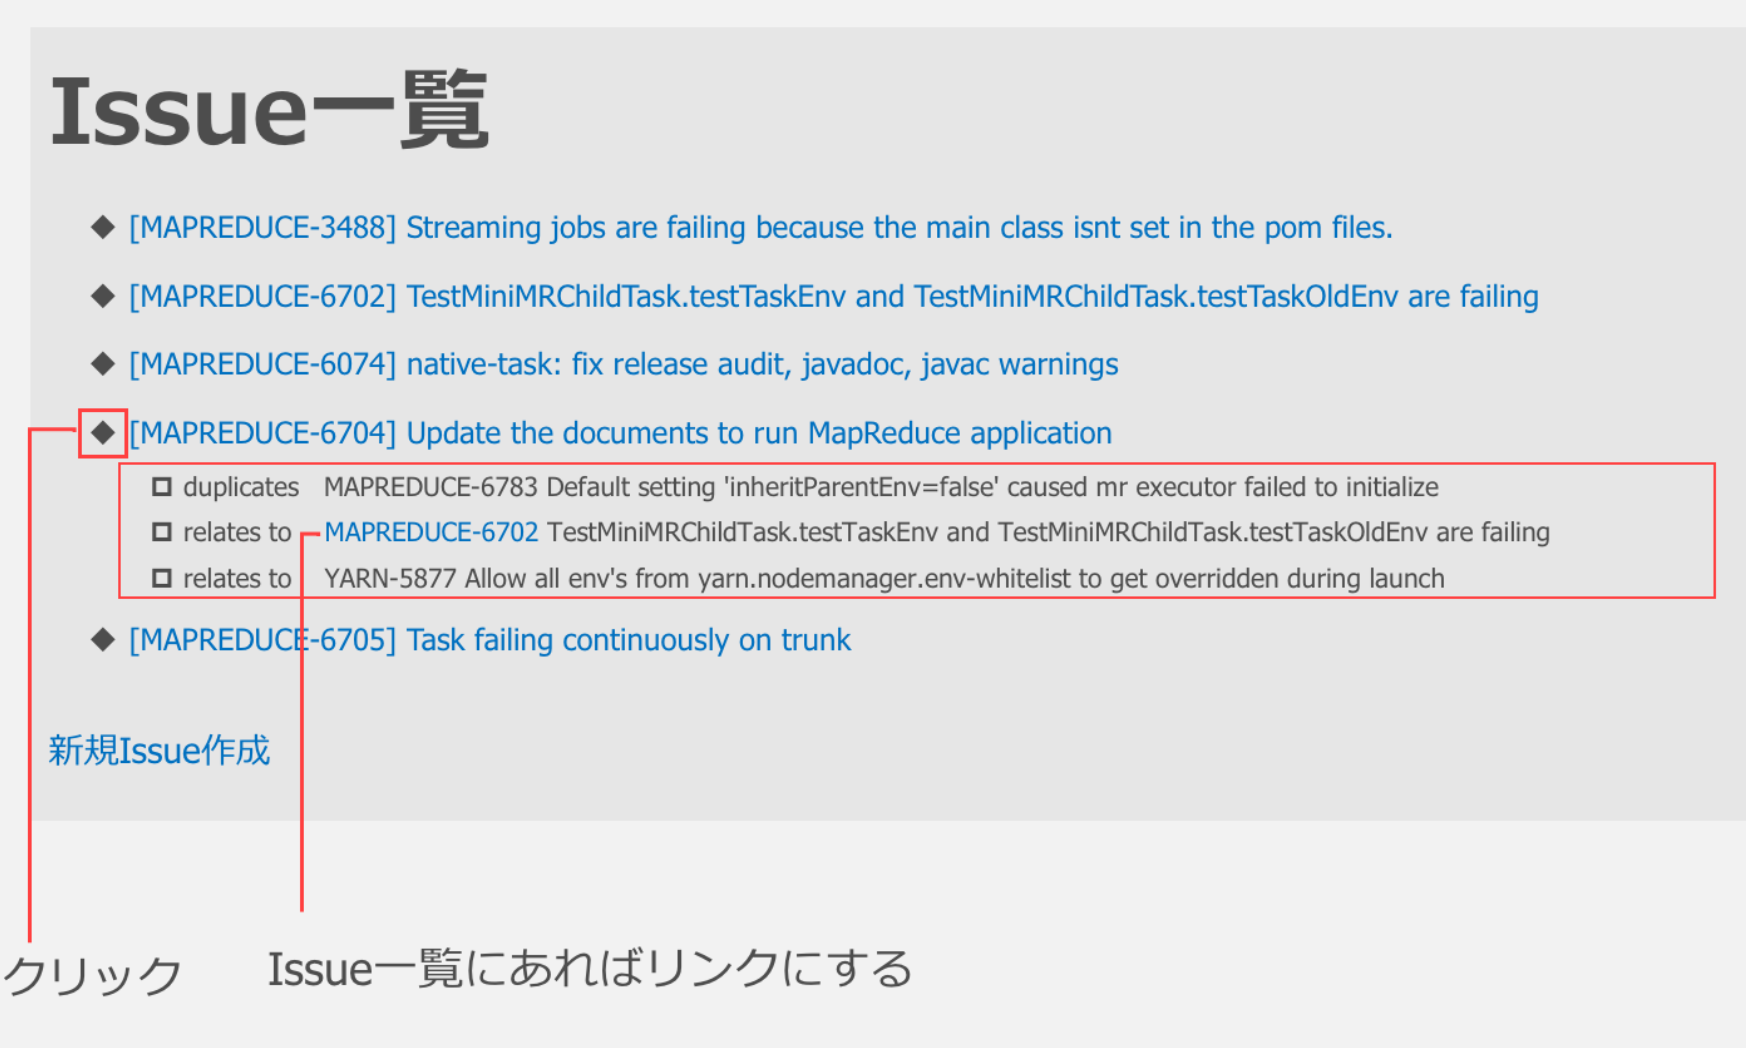
\includegraphics[width=17cm,bb=300 300 -200 27]{RelatesVisualize.png}
		\caption{issue間の関係の可視化}
		\end{figure}
		
		上に示す通り、issue一覧でのそれぞれのissueについて、ひし形のボタンをクリックすると、下にそのissueの関係しているissueを表示するようにしている。また、表示したissueがすでにissue一覧に存在すれば、リンクを貼りそのissueの議論構造に移動することができるようにする。この時、関係しているissueが存在する場合は何らかの方法で関連issueの存在を示すものとする。現状では菱形の横に[関連issue有り]と表示することで示すものとする。

		\subsection{[発展機能] issueごとに担当者・状態の管理}
		ここでは、各issue画面において、issue一つ一つに対して担当者・状態をつけることができるようにする。こうすることで、ユーザーは、そのissueは誰が管理していて、どのような状態であるかを共有することができる。担当者は存在するアカウントのユーザ名の中から選択することができ、状態はこちらでいくつか用意した状態の中から選択する形にする。その情報はissue一覧画面においてissueの横に表示し、確認できるようにする。
		

		\subsection{[発展機能] 議論構造の編集・整理のユーザビリティ向上}
		全ての機能の実装が終わった場合に、実装する機能である。議論構造の編集は現在使いやすいものとは言えない。そのため、いくつかの機能を実装することで、議論構造の編集を簡単なものにする。現状では、議論構造の編集はコメントのノードをクリックした際に出るポップアップからしかできない。なので、議論構造の変更をドラッグなどの使いやすい実装に変えることを考えている。また、議論構造のリセットもできるようにすることで、議論構造を作り直したいときに便利である。他にも議論構造の編集・整理のユーザビリティが向上する実装を適用していくつもりである。

	\section{データベース要求}
	
	以下に、作成する機能に関わる、重要なテーブルとテーブルに設けるカラムを中心に内容を説明する。
	
		\subsection{usersテーブル}
		このテーブルでは、アカウントごとにメールアドレス、ユーザ名、パスワードなどを持つ。
		\begin{itemize}
		\item id
		\item {\bf email (メールアドレス)}
		\item {\bf username (ユーザ名)}
		\item role
		\item {\bf encrypted\_passward (パスワード)}
		\item reset\_password\_token
		\item reset\_password\_sent\_at 
		\item remember\_created\_at
		\item sign\_in\_count
		\item current\_sign\_in\_at
		\item last\_sign\_in\_at
		\item current\_sign\_in\_ip
		\item last\_sign\_in\_ip
		\item created\_at
		\item updated\_at 
		\end{itemize}
				
		\subsection{projectsテーブル}
		新しく作成したテーブルである。プロジェクトごとにプロジェクト名を持つ。
		\begin{itemize}
		\item id
		\item {\bf name (プロジェクト名)}
		\item created\_at
		\item updated\_at
		\end{itemize}
		
		\subsection{issuesテーブル}
		このテーブルでは新しく、タイトルを含まないissue自体の名前 (例、MAPREDUCE-8704) 、プロジェクトid、担当者のユーザid、状態の種類を持つ。
		\begin{itemize}
		\item id
		\item url
		\item type
		\item title (タイトルを含めたissueの名前)
		\item created\_at
		\item updated\_at
		\item {\bf name (issue自体の名前)}
		\item {\bf project\_id (プロジェクトid)}
		\item {\bf user\_id (担当者のユーザid)}
		\item {\bf status\_type (状態の種類)}
		\end{itemize}
				
		\subsection{issue\_relationsテーブル}
		新しく作成したテーブルである。複数issue間の関係の可視化のために用意したもので、どのissueに関する関係なのか、どのような関係があるのかなどの情報を持つ。
		\begin{itemize}
		\item id
		\item {\bf source\_issue\_id (どのissueに関する関係か)}
		\item {\bf target\_issue\_title (関係先のissueのtitle)}
		\item {\bf target\_issue\_ name (関係先のissueのname)}
		\item {\bf type (関係の種類)}
		\item created\_at
		\item updated\_at
		\end{itemize}

		\subsection{commentsテーブル}
		このテーブルでは、所属しているissue、コメントをした議論参加者名、コメントの内容などを持つ。
		\begin{itemize}
		\item id
		\item {\bf issue\_id (コメントの所属するissue)}
		\item {\bf author (コメントをした議論参加者名)}
		\item {\bf content (コメントの内容)}
		\item type
		\item JIRA\_id
		\item internal\_id
		\item created\_at
		\item updated\_at
		\end{itemize}

		\subsection{edgesテーブル}
		このテーブルでは、議論構造において、どのコメントとどのコメントをつないでいるのかなどの情報を持っている。
		\begin{itemize}
		\item id
		\item user\_id
		\item {\bf source\_comment\_id (どのコメントからのedgeなのか)}
		\item {\bf target\_comment\_id (どのコメントへのedgeなのか)}
		\item type
		\item created\_at
		\item updated\_at
		\item reason
		\end{itemize}
		
		\subsection{tagsテーブル}
		このテーブルでは、タグがどのコメントについているのか、タグの内容は何かなどの情報を持っている。
		\begin{itemize}
		\item id
		\item user\_id
		\item {\bf comment\_id (どのコメントについているタグなのか)}
		\item {\bf content (タグの内容)}
		\item created\_at
		\item updated\_at
		\end{itemize}

		\subsection{auto\_tag\_authorsテーブル}
		このテーブルは元々、ツールがコメントをする場合の議論参加者名(botなど)のみを対象としていたテーブルであったが、今回の機能の追加により自動タグ付けをする議論参加者名全体を対象とするテーブルに変更した。そのため、どのようなタグが議論参加者名に対して存在するのか、またプロジェクトごとに議論作者名を登録するため、どのプロジェクトに適用する自動タグ付けなのかなどを情報として持つようにした。
		\begin{itemize}
		\item id
		\item author\_name
		\item created\_at
		\item updated\_at
		\item {\bf tag\_content (自動タグ付けするタグの内容)}
		\item {\bf project\_id (どのプロジェクトに関するものなのか)}
		\end{itemize}

		\subsection{bookmarksテーブル}
		このテーブルでは、元から備わっているブックマーク機能のために、どのコメントに対するブックマークなのかなどを持っている。
		\begin{itemize}
		\item id
		\item user\_id
		\item comment\_id (どのコメントに対するブックマークか)
		\item created\_at
		\item updated\_at
		\end{itemize}
		
		\subsection{その他のテーブル}
		
		そのほかにもいくつかテーブルがあるが、機能に関わるものでは無いのでテーブル名だけ列挙する。
		
		\begin{itemize}
		\item logsテーブル
		\item schema\_migrationsテーブル
		\item versionsテーブル
		\item ar\_internal\_metadataテーブル
		\end{itemize}
	
	\section{ソフトウェア属性}
	
		\subsection{使用性}
		本ツール改良案では、ただ使いやすいものになっていたり多くの機能があることに比べて、複数の人が共同で作業できるツールにすることが求められている。そのため、ユーザビリティにも気を配るが、主としてCSCWに着手しなければならない。そのことを意識した機能の実装順序にもなっている。また、ツール使用者の要求の優先順位も合わせて考慮し、より使いやすいツールを実現する。
		
		\subsection{拡張性}
		まず、本ツールはRuby on RailsでMVCに基づいて設計がされている。このことは拡張性を高める。またCSCWの向上という機能の中で、共同作業支援に関する、別の機能を追加しようとした場合にも柔軟に対応できるようなデータベース設計をする。またもし今後、ITSとしてJIRA以外に対してもこのツールを適用させようとした際に、プロジェクトごとにissueをグルーピングすることで、プロジェクトごとにITSを対応づけることが可能である。
		
		\subsection{移植性}
		本ツールは、元々「DiscussionVisualizer」の実装にも使われていて、広くWebアプリケーション開発に使われているRuby on Railsを使うことで移植性を高める。

\end{document}

%写真の貼り付けテンプレ
\begin{figure}[H]
\centering
\includegraphics[width=17cm,bb=220 300 -200 27]{firstclass.png}
\caption{設計当初のクラス図}
\end{figure}

%ソースコードの貼り付けテンプレ
\begin{lstlisting}[basicstyle=\ttfamily\footnotesize, frame=single, numbers=left]

\end{lstlisting}